% Created by tikzDevice version 0.6.2 on 2014-10-03 02:34:26
% !TEX encoding = UTF-8 Unicode
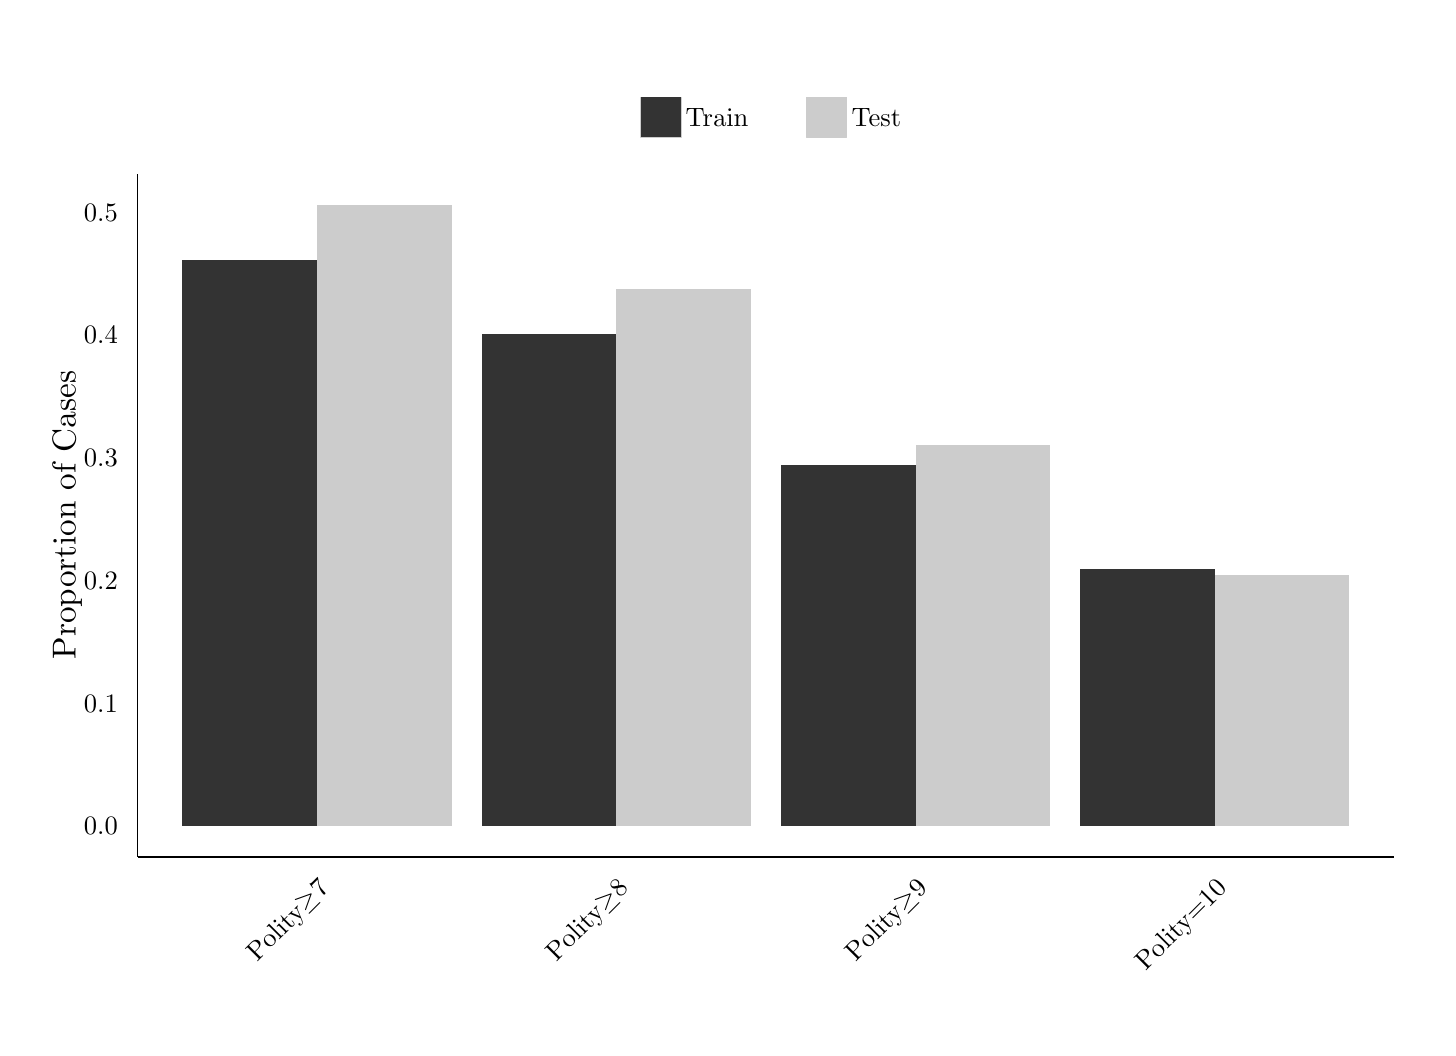
\begin{tikzpicture}[x=1pt,y=1pt]
\definecolor[named]{drawColor}{rgb}{0.00,0.00,0.00}
\definecolor[named]{fillColor}{rgb}{1.00,1.00,1.00}
\fill[color=fillColor,fill opacity=0.00,] (0,0) rectangle (505.89,361.35);
\begin{scope}
\path[clip] (  0.00,  0.00) rectangle (505.89,361.35);
\end{scope}
\begin{scope}
\path[clip] (  0.00,  0.00) rectangle (505.89,361.35);
\end{scope}
\begin{scope}
\path[clip] (  0.00,  0.00) rectangle (505.89,361.35);
\definecolor[named]{drawColor}{rgb}{1.00,1.00,1.00}
\definecolor[named]{fillColor}{rgb}{1.00,1.00,1.00}

\draw[color=drawColor,line width= 0.6pt,line cap=round,line join=round,fill=fillColor,] (  0.00,  0.00) rectangle (505.89,361.35);
\end{scope}
\begin{scope}
\path[clip] (  0.00,  0.00) rectangle (505.89,361.35);
\end{scope}
\begin{scope}
\path[clip] (  0.00,  0.00) rectangle (505.89,361.35);
\end{scope}
\begin{scope}
\path[clip] (  0.00,  0.00) rectangle (505.89,361.35);
\end{scope}
\begin{scope}
\path[clip] ( 39.69, 61.79) rectangle (493.85,308.58);
\definecolor[named]{fillColor}{rgb}{1.00,1.00,1.00}

\draw[fill=fillColor,draw opacity=0.00,] ( 39.69, 61.79) rectangle (493.85,308.58);
\definecolor[named]{fillColor}{rgb}{0.20,0.20,0.20}

\draw[fill=fillColor,draw opacity=0.00,] ( 55.91, 73.01) rectangle (104.57,277.41);
\definecolor[named]{fillColor}{rgb}{0.80,0.80,0.80}

\draw[fill=fillColor,draw opacity=0.00,] (104.57, 73.01) rectangle (153.23,297.36);
\definecolor[named]{fillColor}{rgb}{0.20,0.20,0.20}

\draw[fill=fillColor,draw opacity=0.00,] (164.04, 73.01) rectangle (212.70,250.81);
\definecolor[named]{fillColor}{rgb}{0.80,0.80,0.80}

\draw[fill=fillColor,draw opacity=0.00,] (212.70, 73.01) rectangle (261.36,266.77);
\definecolor[named]{fillColor}{rgb}{0.20,0.20,0.20}

\draw[fill=fillColor,draw opacity=0.00,] (272.17, 73.01) rectangle (320.83,203.36);
\definecolor[named]{fillColor}{rgb}{0.80,0.80,0.80}

\draw[fill=fillColor,draw opacity=0.00,] (320.83, 73.01) rectangle (369.49,210.46);
\definecolor[named]{fillColor}{rgb}{0.20,0.20,0.20}

\draw[fill=fillColor,draw opacity=0.00,] (380.31, 73.01) rectangle (428.97,165.68);
\definecolor[named]{fillColor}{rgb}{0.80,0.80,0.80}

\draw[fill=fillColor,draw opacity=0.00,] (428.97, 73.01) rectangle (477.63,163.46);
\end{scope}
\begin{scope}
\path[clip] (  0.00,  0.00) rectangle (505.89,361.35);
\end{scope}
\begin{scope}
\path[clip] (  0.00,  0.00) rectangle (505.89,361.35);
\definecolor[named]{drawColor}{rgb}{0.00,0.00,0.00}

\draw[color=drawColor,line width= 0.6pt,line join=round,fill opacity=0.00,] ( 39.69, 61.79) --
	( 39.69,308.58);
\end{scope}
\begin{scope}
\path[clip] (  0.00,  0.00) rectangle (505.89,361.35);
\definecolor[named]{drawColor}{rgb}{0.00,0.00,0.00}

\node[color=drawColor,anchor=base east,inner sep=0pt, outer sep=0pt, scale=  0.96] at ( 32.57, 69.70) {0.0};

\node[color=drawColor,anchor=base east,inner sep=0pt, outer sep=0pt, scale=  0.96] at ( 32.57,114.04) {0.1};

\node[color=drawColor,anchor=base east,inner sep=0pt, outer sep=0pt, scale=  0.96] at ( 32.57,158.38) {0.2};

\node[color=drawColor,anchor=base east,inner sep=0pt, outer sep=0pt, scale=  0.96] at ( 32.57,202.72) {0.3};

\node[color=drawColor,anchor=base east,inner sep=0pt, outer sep=0pt, scale=  0.96] at ( 32.57,247.06) {0.4};

\node[color=drawColor,anchor=base east,inner sep=0pt, outer sep=0pt, scale=  0.96] at ( 32.57,291.40) {0.5};
\end{scope}
\begin{scope}
\path[clip] (  0.00,  0.00) rectangle (505.89,361.35);
\end{scope}
\begin{scope}
\path[clip] (  0.00,  0.00) rectangle (505.89,361.35);
\end{scope}
\begin{scope}
\path[clip] (  0.00,  0.00) rectangle (505.89,361.35);
\end{scope}
\begin{scope}
\path[clip] (  0.00,  0.00) rectangle (505.89,361.35);
\end{scope}
\begin{scope}
\path[clip] (  0.00,  0.00) rectangle (505.89,361.35);
\end{scope}
\begin{scope}
\path[clip] (  0.00,  0.00) rectangle (505.89,361.35);
\end{scope}
\begin{scope}
\path[clip] (  0.00,  0.00) rectangle (505.89,361.35);
\definecolor[named]{drawColor}{rgb}{0.00,0.00,0.00}

\draw[color=drawColor,line width= 0.6pt,line join=round,fill opacity=0.00,] ( 39.69, 61.79) --
	(493.85, 61.79);
\end{scope}
\begin{scope}
\path[clip] (  0.00,  0.00) rectangle (505.89,361.35);
\end{scope}
\begin{scope}
\path[clip] (  0.00,  0.00) rectangle (505.89,361.35);
\end{scope}
\begin{scope}
\path[clip] (  0.00,  0.00) rectangle (505.89,361.35);
\definecolor[named]{drawColor}{rgb}{0.00,0.00,0.00}

\node[rotate= 45.00,color=drawColor,anchor=base east,inner sep=0pt, outer sep=0pt, scale=  0.96] at (109.24, 50.00) {Polity$\geq$7};

\node[rotate= 45.00,color=drawColor,anchor=base east,inner sep=0pt, outer sep=0pt, scale=  0.96] at (217.37, 50.00) {Polity$\geq$8};

\node[rotate= 45.00,color=drawColor,anchor=base east,inner sep=0pt, outer sep=0pt, scale=  0.96] at (325.51, 50.00) {Polity$\geq$9};

\node[rotate= 45.00,color=drawColor,anchor=base east,inner sep=0pt, outer sep=0pt, scale=  0.96] at (433.64, 50.00) {Polity$=$10};
\end{scope}
\begin{scope}
\path[clip] (  0.00,  0.00) rectangle (505.89,361.35);
\end{scope}
\begin{scope}
\path[clip] (  0.00,  0.00) rectangle (505.89,361.35);
\end{scope}
\begin{scope}
\path[clip] (  0.00,  0.00) rectangle (505.89,361.35);
\end{scope}
\begin{scope}
\path[clip] (  0.00,  0.00) rectangle (505.89,361.35);
\end{scope}
\begin{scope}
\path[clip] (  0.00,  0.00) rectangle (505.89,361.35);
\end{scope}
\begin{scope}
\path[clip] (  0.00,  0.00) rectangle (505.89,361.35);
\end{scope}
\begin{scope}
\path[clip] (  0.00,  0.00) rectangle (505.89,361.35);
\definecolor[named]{drawColor}{rgb}{0.00,0.00,0.00}

\node[rotate= 90.00,color=drawColor,anchor=base,inner sep=0pt, outer sep=0pt, scale=  1.20] at ( 17.30,185.19) {Proportion of Cases};
\end{scope}
\begin{scope}
\path[clip] (  0.00,  0.00) rectangle (505.89,361.35);
\end{scope}
\begin{scope}
\path[clip] (  0.00,  0.00) rectangle (505.89,361.35);
\end{scope}
\begin{scope}
\path[clip] (  0.00,  0.00) rectangle (505.89,361.35);
\end{scope}
\begin{scope}
\path[clip] (  0.00,  0.00) rectangle (505.89,361.35);
\end{scope}
\begin{scope}
\path[clip] (  0.00,  0.00) rectangle (505.89,361.35);
\end{scope}
\begin{scope}
\path[clip] (  0.00,  0.00) rectangle (505.89,361.35);
\definecolor[named]{fillColor}{rgb}{1.00,1.00,1.00}

\draw[fill=fillColor,draw opacity=0.00,] (213.63,317.45) rectangle (319.90,340.44);
\end{scope}
\begin{scope}
\path[clip] (  0.00,  0.00) rectangle (505.89,361.35);
\end{scope}
\begin{scope}
\path[clip] (  0.00,  0.00) rectangle (505.89,361.35);
\end{scope}
\begin{scope}
\path[clip] (  0.00,  0.00) rectangle (505.89,361.35);
\end{scope}
\begin{scope}
\path[clip] (  0.00,  0.00) rectangle (505.89,361.35);
\definecolor[named]{drawColor}{rgb}{0.80,0.80,0.80}
\definecolor[named]{fillColor}{rgb}{1.00,1.00,1.00}

\draw[color=drawColor,line width= 0.6pt,line cap=round,line join=round,fill=fillColor,] (221.51,321.72) rectangle (235.96,336.17);
\end{scope}
\begin{scope}
\path[clip] (  0.00,  0.00) rectangle (505.89,361.35);
\end{scope}
\begin{scope}
\path[clip] (  0.00,  0.00) rectangle (505.89,361.35);
\definecolor[named]{fillColor}{rgb}{0.20,0.20,0.20}

\draw[fill=fillColor,draw opacity=0.00,] (221.51,321.72) rectangle (235.96,336.17);

\draw[fill opacity=0.00,draw opacity=0.00,] (221.51,321.72) --
	(235.96,336.17);
\end{scope}
\begin{scope}
\path[clip] (  0.00,  0.00) rectangle (505.89,361.35);
\end{scope}
\begin{scope}
\path[clip] (  0.00,  0.00) rectangle (505.89,361.35);
\definecolor[named]{drawColor}{rgb}{0.80,0.80,0.80}
\definecolor[named]{fillColor}{rgb}{1.00,1.00,1.00}

\draw[color=drawColor,line width= 0.6pt,line cap=round,line join=round,fill=fillColor,] (281.46,321.72) rectangle (295.91,336.17);
\end{scope}
\begin{scope}
\path[clip] (  0.00,  0.00) rectangle (505.89,361.35);
\end{scope}
\begin{scope}
\path[clip] (  0.00,  0.00) rectangle (505.89,361.35);
\definecolor[named]{fillColor}{rgb}{0.80,0.80,0.80}

\draw[fill=fillColor,draw opacity=0.00,] (281.46,321.72) rectangle (295.91,336.17);

\draw[fill opacity=0.00,draw opacity=0.00,] (281.46,321.72) --
	(295.91,336.17);
\end{scope}
\begin{scope}
\path[clip] (  0.00,  0.00) rectangle (505.89,361.35);
\end{scope}
\begin{scope}
\path[clip] (  0.00,  0.00) rectangle (505.89,361.35);
\definecolor[named]{drawColor}{rgb}{0.00,0.00,0.00}

\node[color=drawColor,anchor=base west,inner sep=0pt, outer sep=0pt, scale=  0.96] at (237.77,325.64) {Train\qquad\qquad};
\end{scope}
\begin{scope}
\path[clip] (  0.00,  0.00) rectangle (505.89,361.35);
\end{scope}
\begin{scope}
\path[clip] (  0.00,  0.00) rectangle (505.89,361.35);
\definecolor[named]{drawColor}{rgb}{0.00,0.00,0.00}

\node[color=drawColor,anchor=base west,inner sep=0pt, outer sep=0pt, scale=  0.96] at (297.72,325.64) {Test};
\end{scope}
\begin{scope}
\path[clip] (  0.00,  0.00) rectangle (505.89,361.35);
\end{scope}
\begin{scope}
\path[clip] (  0.00,  0.00) rectangle (505.89,361.35);
\end{scope}
\begin{scope}
\path[clip] (  0.00,  0.00) rectangle (505.89,361.35);
\end{scope}
\begin{scope}
\path[clip] (  0.00,  0.00) rectangle (505.89,361.35);
\end{scope}
\begin{scope}
\path[clip] (  0.00,  0.00) rectangle (505.89,361.35);
\end{scope}
\begin{scope}
\path[clip] (  0.00,  0.00) rectangle (505.89,361.35);
\end{scope}
\begin{scope}
\path[clip] (  0.00,  0.00) rectangle (505.89,361.35);
\end{scope}
\begin{scope}
\path[clip] (  0.00,  0.00) rectangle (505.89,361.35);
\end{scope}
\begin{scope}
\path[clip] (  0.00,  0.00) rectangle (505.89,361.35);
\end{scope}
\begin{scope}
\path[clip] (  0.00,  0.00) rectangle (505.89,361.35);
\end{scope}
\begin{scope}
\path[clip] (  0.00,  0.00) rectangle (505.89,361.35);
\end{scope}
\begin{scope}
\path[clip] (  0.00,  0.00) rectangle (505.89,361.35);
\end{scope}
\end{tikzpicture}
